% --- IMPORTS ---
\documentclass[leqno]{article}
\usepackage{graphicx}
\usepackage{dsfont}
\usepackage{mathtools}
\usepackage{amssymb}
\usepackage{amsmath}
\usepackage{amsthm}
\usepackage{float}
\usepackage{ragged2e}
\usepackage{tensor}
\usepackage{fancyhdr}
\usepackage{empheq}
\usepackage[most]{tcolorbox}
\usepackage{enumitem}
\usepackage{dirtytalk}
\usepackage{marginnote}
\usepackage{microtype}
\usepackage[
  a4paper,
  left=0.8in,
  right=1in,
  top=1in,
  bottom=0.5in,
  headheight=14pt,
  headsep=0.4in
]{geometry}
\setlength{\parindent}{0cm}
% --- TikZ Packages ---
\usepackage{pgfplots}
\pgfplotsset{compat=1.18}
\usepgfplotslibrary{fillbetween, polar}
\usetikzlibrary{calc, positioning}
\usetikzlibrary{angles, quotes}
\usetikzlibrary{arrows.meta}
\usetikzlibrary{decorations.pathreplacing, decorations.markings}
\usetikzlibrary{patterns}
\usetikzlibrary{intersections}
% --- URL Packages ---
\usepackage[colorlinks=true,linkcolor=red,citecolor=magenta,urlcolor=black]{hyperref}%
\urlstyle{same}
% --- END OF IMPORTS ---

% --- CUSTOM COMMANDS ---
\RenewDocumentCommand{\marks}{o m}{%
  \IfValueTF{#1}%
    {\marginnote{\raggedright\textbf{[#2]}}[#1]}%
    {\marginnote{\raggedright\textbf{[#2]}}}%
}
\newcommand{\vspacerule}[2]{%
  \par\vspace*{#1}%
  \noindent\hrulefill\par
  \vspace*{#2}%
}
\definecolor{scarlet}{RGB}{205, 40, 75}
\newcommand{\questionitem}{%
  \item\phantomsection
  \addcontentsline{toc}{section}{Question \number\value{enumi}}%
}
\renewcommand{\contentsname}{Questions}
% --- END OF CUSTOM COMMANDS ---

% --- HEADER CONFIG ---
\pagestyle{fancy}
\fancyhead{}
\fancyfoot{}
\renewcommand{\headrulewidth}{0.9pt}
\lhead{Modelling with 2nd Order Differential Equations}
\chead{}
\rhead{\href{https://danieljsmith.org}{danieljsmith.org}}
% --- END OF HEADER CONFIG ---

\begin{document}
\vspace*{20pt}
\tableofcontents
\newpage
\begin{enumerate}[
  label=\textbf{\arabic*.},
  leftmargin=*,
  topsep=0pt,
  partopsep=0pt,
  parsep=0pt
]


% ---- Question 1 ----
\questionitem
% [Source: _QBT__Modelling_with_2nd_Order_Differential_Equations, Q1]

\begin{figure}[H]
    \centering
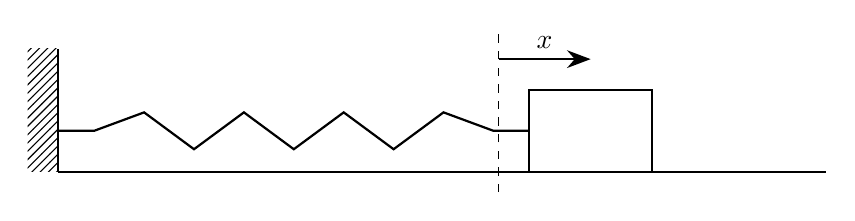
\begin{tikzpicture}[scale=1.3]
\def\wallx{-3.2}
\def\eqx{1.1}
\def\disp{0.9}
\def\bw{1.2}
\def\bh{0.8}
\pgfmathsetmacro{\midy}{\bh/2}
\pgfmathsetmacro{\cx}{\eqx+\disp}
\pgfmathsetmacro{\leftx}{\cx-\bw/2}
\pgfmathsetmacro{\rightx}{\cx+\bw/2}
\pgfmathsetmacro{\lead}{0.35}
\pgfmathsetmacro{\amp}{0.18}
\pgfmathsetmacro{\coilstart}{\wallx+\lead}
\pgfmathsetmacro{\coilend}{\leftx-\lead}
\pgfmathsetmacro{\step}{(\coilend-\coilstart)/8}
\pgfmathsetmacro{\arrowy}{\bh+0.3}
\pgfmathsetmacro{\marktop}{\bh+0.55}

\fill[pattern=north east lines] (\wallx-0.3,0) rectangle (\wallx,1.2);
\draw[thick] (\wallx,0) -- (\wallx,1.2);
\draw[thick] (\wallx,0) -- (4.3,0);

\draw[thick] (\wallx,\midy) -- (\coilstart,\midy)
  -- ++(\step,\amp) -- ++(\step,{-2*\amp}) -- ++(\step,{2*\amp})
  -- ++(\step,{-2*\amp}) -- ++(\step,{2*\amp}) -- ++(\step,{-2*\amp})
  -- ++(\step,{2*\amp}) -- ++(\step,{-\amp}) -- (\leftx,\midy);

\draw[thick] (\leftx,0) rectangle (\rightx,\bh);
\draw[dashed] (\eqx,-0.2) -- (\eqx,\marktop);
\draw[-{Stealth[length=3mm]}, thick] (\eqx,\arrowy) -- (\cx,\arrowy) node[midway, above] {$x$};
\end{tikzpicture}
\end{figure}


The horizontal displacement of a glider attached to a spring, shown in the diagram above, is modelled by the differential equation \\
\[\frac{\mathrm{d}^2 x}{\mathrm{d} t^2}+16x=3\sin 4t\] \\
where $x$ is the displacement, in metres, of the glider from its equilibrium position, $t$ seconds after the motion begins. \\
\begin{enumerate}[label=\textbf{(\alph*)}]
  \item
  \begin{enumerate}[label=(\roman*)]
    \item Show that a particular solution of the differential equation is
    \[
    x=-\frac{3}{8} t \cos 4t
    \] \marks[-20pt]{4}
    \item Hence, find the general solution of the differential equation \marks{4} \\
  \end{enumerate}
\end{enumerate}
Initially, the glider is $0.20\,\mathrm{m}$ to the right of equilibrium and is moving towards equilibrium at $0.50\,\mathrm{m\,s^{-1}}$. \\
Given that, $4$ seconds after the motion begins, the displacement of the glider is $\beta$ m, \\
\begin{enumerate}[label=\textbf{(\alph*)}, resume]
  \item determine, according to the model, the value of $\beta$ to $3$ significant figures \marks{4} \\
  \item Given that the true value of $\beta$ is $0.46\,\mathrm{m}$, comment on the suitability of the model \marks{1} \\
  \item Write down a differential equation for the glider if the periodic driving force is removed, so that the motion becomes simple harmonic \marks{1} \\
\end{enumerate}

\newpage

% ---- Question 2 ----
\questionitem
% [Source: _QBT__Modelling_with_2nd_Order_Differential_Equations, Q2]

\begin{figure}[H]
    \centering
\begin{tikzpicture}[scale=1.3]
\def\lineL{3.8}
\def\pos{2.6}
\def\velLen{1.25}
\def\forceLen{1.25}
\def\dispY{0.75}

\coordinate (O) at (0,0);
\coordinate (P) at (\pos,0);

\draw[thick, dashed] (-\lineL,0) -- (P);
\draw[thick] ($(O)+(0,-0.18)$) -- ($(O)+(0,0.18)$);
\node[above] at ($(O)+(0,0.15)$) {$O$};

\fill (P) circle (2.8pt);

\draw[-{Stealth[length=3mm]}, thick]
    ($(P)+(0.75,0.65)$) -- ++(-\velLen,0)
    node[midway, above, xshift=5pt] {$v\,\mathrm{m\,s^{-1}}$};

\draw[-{Stealth[length=3mm]}, thick]
    ($(P)+(1.50,0)$) -- ++(-\forceLen,0)
    node[midway, below, xshift=5pt] {$9mx\,\mathrm{N}$};

\draw[-{Stealth[length=3mm]}, thick]
    ($(O)+(0,-\dispY)$) -- ($(P)+(0,-\dispY)$)
    node[midway, below] {$x\,\mathrm{m}$};
\end{tikzpicture}
\end{figure}


A particle of mass $m\,\mathrm{kg}$ moves in a horizontal line through its equilibrium position $O$. At time $t$ seconds its displacement from $O$ is $x$ metres and its speed is $v\,\mathrm{m\,s^{-1}}$. When the particle is to the right of $O$, it is acted on by a restoring force of magnitude $9mx$ newtons directed towards $O$, as shown in the diagram. \\

At $t=0$, the particle is $1$ m to the right of $O$ and is projected towards $O$ with speed $6\,\mathrm{m\,s^{-1}}$. \\

\begin{enumerate}[label=\textbf{(\alph*)}]
  \item In the absence of damping and any external force,
  \begin{enumerate}[label=(\roman*)]
    \item Show that the motion is modelled by the differential equation
    \[
    \frac{\mathrm{d}^2 x}{\mathrm{d} t^2}+9x=0
    \] \marks[-20pt]{1}
    \item State the type of motion \marks{1}
    \item Write down the period of the motion \marks{1}
    \item Find $x$ in terms of $t$ \marks{4}
    \item Find the amplitude of the motion \marks{2} \\
  \end{enumerate}
  \item In a second model, the particle again starts from the same initial position and velocity, but the motion is damped by a force $6mv$ newtons acting opposite to the direction of motion. \\
  \begin{enumerate}[label=(\roman*)]
    \item Show that
    \[
    \frac{\mathrm{d}^2 x}{\mathrm{d} t^2}+6\frac{\mathrm{d} x}{\mathrm{d} t}+9x=0
    \] \marks[-20pt]{1}
    \item State, giving a reason, whether the system is under-damped, critically damped or over-damped \marks{1}
    \item Determine the general solution of this differential equation \marks{3} \\
  \end{enumerate}
  \item In a third model, the particle again starts from the same initial position and velocity, and is subject both to the damping force in part (b) and to an external force $25m\cos 4t$ newtons acting in the positive direction. The motion is now modelled by the differential equation
  \[
  \frac{\mathrm{d}^2 x}{\mathrm{d} t^2}+6\frac{\mathrm{d} x}{\mathrm{d} t}+9x=25\cos 4t
  \]
  \begin{enumerate}[label=(\roman*)]
    \item Find $x$ in terms of $t$ \marks{7} \\
    \item In the long term, the particle is observed to perform simple harmonic motion with period about $1.6$ seconds. Verify that this is consistent with the answer to part (c)(i) \marks{2} \\
  \end{enumerate}
\end{enumerate}

\newpage

% ---- Question 3 ----
\questionitem
% [Source: _QBT__Modelling_with_2nd_Order_Differential_Equations, Q3]

The charge $q$ on a capacitor in a driven RLC circuit is modelled by \\
\[\frac{\mathrm{d}^2 q}{\mathrm{d} t^2}+2\frac{\mathrm{d} q}{\mathrm{d} t}+10q=37\cos 3t\] \\
where $t\geq0$ is time. \\

When $t=0$, $q=1$ and $\frac{\mathrm{d} q}{\mathrm{d} t}=15$. \\

\begin{enumerate}[label=\textbf{(\alph*)}]
  \item Find $q$ as a function of $t$ \marks{9} \\
  \item Hence write down an approximate expression for $q$ when $t$ is large, giving your answer in the form $R\cos(3t-\alpha)$, where $R>0$ and $0<\alpha<\frac{\pi}{2}$ \marks{4} \\
\end{enumerate}

\newpage

% ---- Question 4 ----
\questionitem
% [Source: _QBT__Modelling_with_2nd_Order_Differential_Equations, Q4]

The vertical displacement of the body of a car from its steady running height is measured by $y$ metres, where $y$ is positive upwards. The body can move above or below this level, so $y$ can take positive and negative values. After the car leaves a speed hump, the body is momentarily above its steady running height and at rest at time $t=0$. \\

A proposed model for the subsequent motion, for $t\ge 0$, is
\[
4\frac{\mathrm{d}^2 y}{\mathrm{d} t^2}+p\frac{\mathrm{d} y}{\mathrm{d} t}+9y=0,
\]
where $p$ is a constant and $p\ge 0$. \\

\begin{enumerate}[label=\textbf{(\alph*)}]
  \item
  \begin{enumerate}[label=(\roman*)]
    \item According to the model, for what value of $p$ would the motion be simple harmonic? \marks{1}
    \item Explain briefly why modelling the motion as simple harmonic is unlikely to be realistic for a car suspension \marks{1} \\
  \end{enumerate}
  \item Find the range of values of $p$ for which the model predicts that the body of the car never goes below its steady running height \marks{2} \\
  \item Sketch a possible graph of $y$ against $t$ when $p$ lies outside the range found in part (b) but the motion is not simple harmonic \marks{1} \\
\end{enumerate}

\newpage

% ---- Question 5 ----
\questionitem
% [Source: _QBT__Modelling_with_2nd_Order_Differential_Equations, Q5]

A load of mass $m\,\mathrm{kg}$ hangs from a light vertical spring and is free to move only vertically in a liquid. \\

The spring has spring constant $k\,\mathrm{N\,m^{-1}}$, and the liquid exerts a resistance force of magnitude $c v$ newtons opposite to the direction of motion, where $v\,\mathrm{m\,s^{-1}}$ is the speed of the load. \\

Let $y$ metres be the downward displacement of the load from its equilibrium position at time $t$ seconds. Assume that $4km>c^2$. \\

\begin{enumerate}[label=\textbf{(\alph*)}]
  \item Show that the motion is modelled by
  \[
  m\frac{\mathrm{d}^2 y}{\mathrm{d} t^2}+c\frac{\mathrm{d} y}{\mathrm{d} t}+ky=0
  \]
  and hence show that
  \[
  y=\mathrm{e}^{-\frac{c t}{2m}}\left(P\cos\left(\frac{\sqrt{4km-c^2}}{2m}\,t\right)+Q\sin\left(\frac{\sqrt{4km-c^2}}{2m}\,t\right)\right),
  \]
  where $P$ and $Q$ are constants. \marks[-30pt]{7} \\
  \item It is given that
  \[
  \renewcommand{\arraystretch}{1.2}
  \begin{array}{rcl}
  m&=&5\\
  c&=&30\\
  k&=&125
  \end{array}
  \]
  At time $t=0$, the load is $0.12\,\mathrm{m}$ below its equilibrium position and is moving upwards with speed $0.12\,\mathrm{m\,s^{-1}}$. \\
  \begin{enumerate}[label=(\roman*)]
    \item Find the values of $P$ and $Q$ \marks{4}
    \item Find the first positive value of $t$ for which the load is at its equilibrium position \marks{5} \\
  \end{enumerate}
  \item A second model ignores the resistance force but keeps the same values of $m$ and $k$. Using the same initial conditions as in part (b), find an expression for $y$ in terms of $t$, giving numerical constants to two significant figures where appropriate \marks{6} \\
\end{enumerate}

\newpage

% ---- Question 6 ----
\questionitem
% [Source: _QBT__Modelling_with_2nd_Order_Differential_Equations, Q6]

A manufacturer is testing the response of an electronic weighing platform. The displayed mass, $m$, measured in kilograms, after a box is placed on the platform is modelled by the differential equation \\
\[4\frac{\mathrm{d}^2 m}{\mathrm{d} t^2}+4\frac{\mathrm{d} m}{\mathrm{d} t}+5m=20\] \\
where $t$ is the number of seconds after the box is placed on the platform. \\

\begin{enumerate}[label=\textbf{(\alph*)}]
  \item Find a general solution of the differential equation \marks{4} \\
\end{enumerate}
Initially, the display reads $0$ kg and the displayed mass is increasing at $5\,\mathrm{kg\,s^{-1}}$. \\
\begin{enumerate}[label=\textbf{(\alph*)}, resume]
  \item Find, according to the model, the greatest value shown on the display \marks{8} \\
\end{enumerate}
The machine is programmed to print a label only when the displayed mass is less than $4.05$ kg. \\
\begin{enumerate}[label=\textbf{(\alph*)}, resume]
  \item Determine whether, according to the model, the machine will print a label exactly $8$ seconds after the box is placed on the platform \marks{2} \\
\end{enumerate}

\newpage

% ---- Question 7 ----
\questionitem
% [Source: _QBT__Modelling_with_2nd_Order_Differential_Equations, Q7]

An analogue meter has a damped pointer. After a short electrical pulse, the angular displacement $\theta$ radians of the pointer from its rest position, measured positive clockwise, is modelled by \\
\[\frac{\mathrm{d}^2 \theta}{\mathrm{d} t^2}+5\frac{\mathrm{d} \theta}{\mathrm{d} t}+6\theta=4\mathrm{e}^{-4t}\] \\
where $t$ is the time, in seconds, after the motion begins. \\

In one test, at $t=0$ the pointer is passing through its rest position and has angular velocity $1\,\mathrm{rad\,s^{-1}}$ anticlockwise. \\

For this test, use the model to
\begin{enumerate}[label=\textbf{(\alph*)}]
  \item find an equation for $\theta$ in terms of $t$ \marks{8} \\
  \item find, to $3$ decimal places, the greatest clockwise angular displacement of the pointer from its rest position \marks{4} \\
\end{enumerate}
In this test, the time taken for the pointer to pass through its rest position again was measured as $0.69$ seconds. \\
\begin{enumerate}[label=\textbf{(\alph*)}, resume]
  \item State, with justification, whether or not this supports the model \marks{1} \\
\end{enumerate}

\newpage

% ---- Question 8 ----
\questionitem
% [Source: _QBT__Modelling_with_2nd_Order_Differential_Equations, Q8]

A trolley moves on a horizontal track and is attached to a spring and a dashpot. The trolley is pulled to the right of its equilibrium position and released. \\

At time $t$ seconds after release, its horizontal displacement is $x$ metres to the right of a fixed point $P$, where $P$ is the equilibrium position and is $1.2$ metres from the left-hand end of the track. \\

When $t=0$:
\[
\renewcommand{\arraystretch}{1.2}
\begin{array}{l}
x=0.18,\\
\text{the velocity of the trolley is }0\,\mathrm{m\,s^{-1}},\\
\text{the acceleration of the trolley is }-0.10\,\mathrm{m\,s^{-2}}
\end{array}
\] \\
In the subsequent motion, the displacement of the trolley is modelled by the differential equation
\[
3k\frac{\mathrm{d}^2 x}{\mathrm{d} t^2}+2k\frac{\mathrm{d} x}{\mathrm{d} t}+5x=0,\qquad t\ge 0,
\]
where $k$ is a positive constant. \\

\begin{enumerate}[label=\textbf{(\alph*)}]
  \item Find the value of $k$ \marks{2} \\
  \item Find the particular solution of the differential equation \marks{7} \\
  \item Hence find, according to the model, the distance of the trolley from the left-hand end of the track $4.5$ seconds after it is released \marks{2} \\
  \item State one limitation of the model \marks{1} \\
\end{enumerate}

\newpage

% ---- Question 9 ----
\questionitem
% [Source: _QBT__Modelling_with_2nd_Order_Differential_Equations, Q9]

In a feedback system, the error signal $E$ is measured in suitable units. \\

For $t\ge 0$, $E$ is modelled by the differential equation
\[\frac{\mathrm{d}^2 E}{\mathrm{d} t^2}+\frac{\mathrm{d} E}{\mathrm{d} t}-6E=-12\] \\
Initially the error is decreasing at $9$ units per second, so $\frac{\mathrm{d} E}{\mathrm{d} t}=-9$ when $t=0$. It is given that $E$ tends to a finite limit as $t\to\infty$. \\

\begin{enumerate}[label=\textbf{(\alph*)}]
  \item Determine the value of $E$ when $t=\ln 2$ \marks{6} \\
  \item Determine the limit of $E$ as $t\to\infty$ \marks{1} \\
\end{enumerate}

\newpage

% ---- Question 10 ----
\questionitem
% [Source: _QBT__Modelling_with_2nd_Order_Differential_Equations, Q10]

A machine part executes damped forced vibrations. Its displacement $y$ centimetres from equilibrium at time $t$ seconds is modelled by \\
\[
\frac{\mathrm{d}^2 y}{\mathrm{d}t^2}+2\frac{\mathrm{d}y}{\mathrm{d}t}+10y=20\cos t+5\sin t,\qquad t\ge 0
\] \\
\begin{enumerate}[label=\textbf{(\alph*)}]
  \item Find the general solution of this differential equation. \marks{6} \\
  \item Given that $y=3$ and $\frac{\mathrm{d}y}{\mathrm{d}t}=3$ when $t=0$, find the particular solution describing the motion. \marks{4} \\
  \item The first turning point of this motion for $t>0$ occurs when $y=a$. Find $a$ correct to $3$ significant figures. \marks{4} \\
\end{enumerate}

\newpage

% ---- Question 11 ----
\questionitem
% [Source: _QBT__Modelling_with_2nd_Order_Differential_Equations, Q11]

A particle $Q$ moves along the $x$-axis under a single force. When the time is $t$ seconds, the displacement of $Q$ from the origin is $x$ metres and its velocity is $v\,\mathrm{m\,s^{-1}}$. \\

The motion of $Q$ is modelled by the differential equation \[\ddot{x}+\lambda^2 x=0\] where $\lambda\,\mathrm{rad\,s^{-1}}$ is a positive constant. \\

At time $t=0$, $Q$ is at the point $A$ where $x=-\tfrac{1}{2}a$, for some positive constant $a$, and is moving in the positive direction. \\

Later, $Q$ reaches the point $B$ where $x=a$ and comes to instantaneous rest. \\
\begin{enumerate}[label=\textbf{(\alph*)}]
  \item Write down the general solution of this differential equation. \marks{1}
  \item Using the answer to part (a), determine expressions, in terms of $\lambda$, $a$ and $t$ only, for the following quantities:
  \begin{enumerate}[label=(\roman*)]
    \item $x$
    \item $v$
  \end{enumerate}
  \marks[-20pt]{3}
  \item Hence show that
  \[ v^2=\lambda^2\bigl(a^2-x^2\bigr) \]
  \marks[-20pt]{1}
  \item The quantity $r$ is defined by $r=\dfrac{1}{v}$. Using part (c), determine an expression for $r_m$, the mean value of $r$ with respect to the displacement, as $Q$ moves directly from $A$ to $B$. \marks{4}
  \item One measure of the validity of the model is consideration of the value of $r_m$. If $r_m$ exceeds $7.2$ then the model is considered to be valid. The value of $a$ is measured as $0.240$ to $3$ significant figures. The value of $\lambda$ is measured as $0.80\pm 0.02$. Determine what can be inferred about the validity of the model from the given information. \marks{1}
  \item Find, according to the model, the least possible value of the velocity of $Q$ at time $t=0$. Give your answer to $2$ significant figures. \marks{2}
\end{enumerate}

\newpage


% ---- Question 12 ----
\questionitem
% [Source: _QBT__Modelling_with_2nd_Order_Differential_Equations, Q12]

An automated inspection trolley of mass $2\,\mathrm{kg}$ moves along a straight horizontal rail. The point $A$ is fixed on the rail. The displacement of the trolley from $A$ at time $t$ seconds is $x$ metres, for $t\ge 0$. \\

For the interval considered, the trolley stays to the right of $A$ and continues to move away from $A$. \\

For $t\ge 0$, the trolley is subject to three forces modelled as follows: \\

- A driving force of magnitude $4(t+1)\,\mathrm{N}$ acts in the positive $x$-direction. \\[2.5pt]
- A magnetic force of magnitude $x\,\mathrm{N}$ acts towards $A$. \\[2.5pt]
- A resistive force of magnitude $2\left|\tfrac{\mathrm{d}x}{\mathrm{d}t}\right|\,\mathrm{N}$ acts opposite to the direction of motion. \\

\begin{enumerate}[label=\textbf{(\alph*)}]
  \item Applying Newton's second law gives the differential equation
  \[
  4(t+1)-x-2\frac{\mathrm{d}x}{\mathrm{d}t}=2\frac{\mathrm{d}^2 x}{\mathrm{d} t^2}
  \]
  \begin{enumerate}[label=(\roman*)]
    \item Explain the sign of the term involving $\frac{\mathrm{d}x}{\mathrm{d}t}$ in this differential equation \marks{1}
    \item When $t=0$ the displacement of the trolley is $1\,\mathrm{m}$, and it is moving away from $A$ with speed $1\,\mathrm{m\,s^{-1}}$. Without attempting to solve the differential equation, find the acceleration of the trolley when $t=0$ \marks{2} \\
  
  \end{enumerate}
  \item Let the particular solution to the differential equation in part (a) be a function $g$ such that $x=g(t)$ for $t\ge 0$. The particular solution can be expressed as a Maclaurin series. \\
  \begin{enumerate}[label=(\roman*)]
    \item Show that the Maclaurin series for $g(t)$ up to and including the term in $t$ is $1+t$ \marks{1}
    \item Use your answer to part (a)(ii) to show that the term in $t^2$ in the Maclaurin series for $g(t)$ is $\frac{1}{4}t^2$ \marks{1}
    \item By differentiating the differential equation in part (a) with respect to $t$, show that the term in $t^3$ in the Maclaurin series for $g(t)$ is $\frac{1}{6}t^3$ \marks{4} \\
  \end{enumerate}
  \item You are given that the complete Maclaurin series for the function $g$ is valid for all $t\ge 0$. After $0.4$ seconds a sensor records that the trolley is $1.45\,\mathrm{m}$ from $A$. \\
  \begin{enumerate}[label=(\roman*)]
    \item Using the Maclaurin series for $g(t)$ up to and including the term in $t^3$, evaluate the suitability of the model for determining the displacement of the trolley from $A$ when $t=0.4$ \marks{1} \\
    
    \item Explain why it would not be sensible to use the Maclaurin series for $g(t)$ up to and including the term in $t^3$ to evaluate the suitability of the model for determining the displacement of the trolley from $A$ when $t=8$ \marks{1} \\
  \end{enumerate}
\end{enumerate}

\end{enumerate}
\end{document}
